\lhead{Theory}
The literature discussed in the previous chapter provides a base for Synthsonic. While SMOTE is easy to use and GANs are very successful at generating images and sound, there is still room for a probabilistic model for synthesizing tabular data due to the limitations of regular SMOTE-based oversamplers and the difficulties of GANs.

\section{Synthsonic}
This section is dedicated to the theory behind Synthsonic. Contrary to other techniques such as SMOTE or other generative algorithms, Synthsonic uses reversible mathematical transformations, making use of as much information in the dataset as possible. This has the additional benefit that Synthsonic is easier to interpret than other GANs, where the synthesis of new samples happens through convolutional neural networks. Additionally, 


Synthsonic consists out of multiple reversible transformations of features. It can handle both numerical and categorical features, and will split a dataset $X$ into a numerical and categorical set, so that $X = (X_{num}, X_{cat})$. Modelling of the dataset happens in five steps:

\begin{enumerate}
    \item Numerical features are transformed into uniformly distributed ones, using reversible steps, from which the first-order correlations have been removed.
    \item Categorical and discretized numerical features are jointly modelled with a Bayesian network.
    \item Specific features can be selected for additional modelling.
    \item A discriminative learner is trained to model the residual discrepancies observed between the input data and the Bayesian network.
    \item The discriminative learner is calibrated to reweigh samples from the Bayesian network.
\end{enumerate}

Each of these steps will be discussed over the following sections.

\section{Feature transformations}
\label{sec:Feat_trans}
The numerical features in $X_{num}$ are transformed from their original distribution to a uniform distribution in three quantile transformations. These steps are performed on each numerical feature $j$. In the first step, a small part of white noise is added to each numerical value in order to ensure a smooth transformation to a normal distribution $X_{normal}$. The process can be described using an inverse Jacobian, with normal density distribution $G(X)$ and the marginalized probability density function $f_j(X_{num}[j])$, where $X_{num}[j]$ is the original feature. 

\begin{equation}
    \prod_{j} \frac{f_j(X_{num}[j])}{G(X_{normal}[j])}
\end{equation}

The next step is to perform a PCA rotation on $X_{normal}$, while keeping the same number of features. Any linear correlations are then removed from the data resulting in a new dataset $X_{pc}$. The principal components do not need to follow a normal distribution when non-linear dependencies are present.

Lastly, the individual features $j$ in $X_{pc}$ are again quantile transformed into a uniform distribution with range (0,1). Again, this can be described by an inverse Jacobian using the marginalized probability density function $k_i(X_{pc}[i]$

\begin{equation}
    \prod_j k_j (X_{pc}[j])
\end{equation}

This three step process removes the linear dependencies but non-linear ones are still present, nor have the categorical features been handled. The final result of this process is now $X_{uniform}$.

\section{Bayesian Network}
The next step is to combine the previously transformed numerical features with the categorical features. As mentioned in the literature review, Bayesian Networks are useful when dealing with discrete, conditional features. However, treating $X_{cat}$ and $X_{uniform}$ separately would mean that any relation or dependency between these sets would not be captured when modelling the data and potentially miss important information. To counter this, features from $X_{uniform}$ are discretized into 20 equally sized bins in the same range of (0,1) to form $X_{discrete}$. Combining this with $X_{cat}$ gives a fully discrete dataset $X_{bn} = (X_{cat}, X_{discrete})$ with the same shape as the original dataset $X$. A standard tree-based Bayesian Network can then be modelled to describe the dependencies within and between all features~\cite{Chow1968ApproximatingTrees}.

\section{Discriminative learning}
The Bayesian Network has modelled the dependencies between all features, but non-linear correlations can still be present. A classifier is used to model this last part of dependency. A new set is introduced, $X_{trans} = (X_{cat},X_{uniform}$, and is split into a 70\%/30\% train/test split. Then a sample of size $X_{trans}$ is generated from the Bayesian Network, called $X_{syn}$. The samples then receive a class label, where $X_{trans}$ is class 1 and $X_{syn}$ is class 0. The default classifier in synthsonic is XGBoost~\cite{Chen2016XGBoost:System}, and is trained to distinguish between the original training data $X_{trans}$ and the generated sample $X_{syn}$. The closer $X_{syn}$ is to the original distribution, the harder it is for the classifier to distinguish between a real and generated sample. However, if it manages to separate them, a better model must be formed. 

\begin{figure}[htp]
\centering
\begin{subfigure}{0.3\textwidth}
\centering
    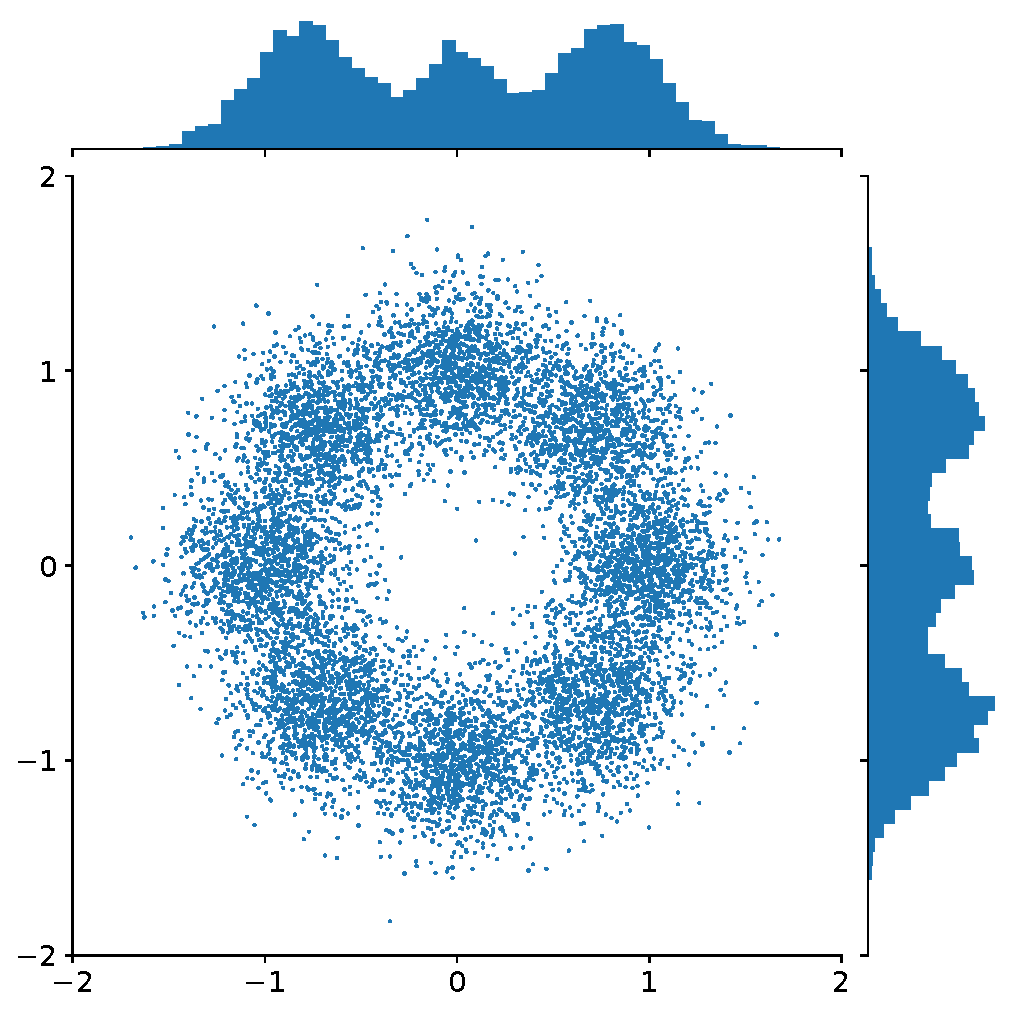
\includegraphics[width=\textwidth]{../Plots/Transformations/ring_joint_marginal_data.pdf}\quad
\caption{$X_{num}$}
\end{subfigure}
\begin{subfigure}{0.3\textwidth}
\centering
    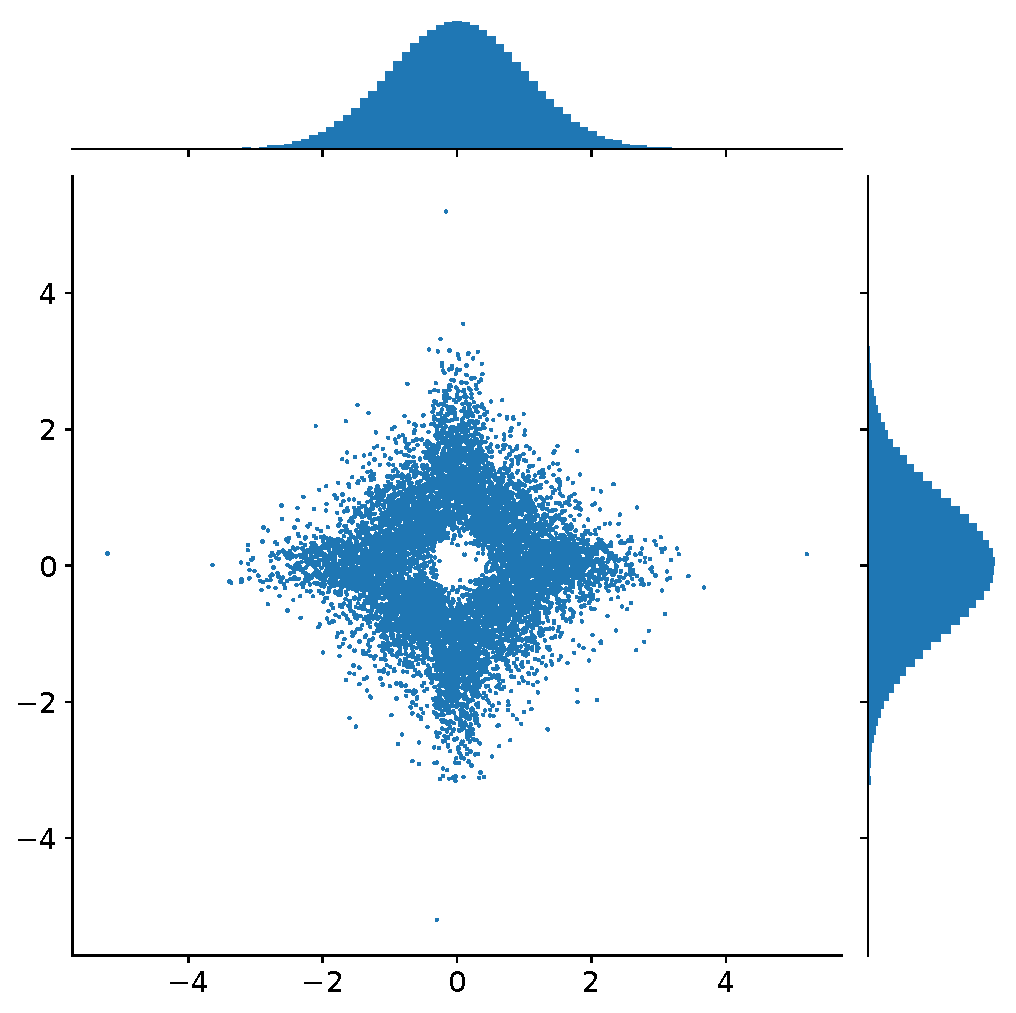
\includegraphics[width=\textwidth]{../Plots/Transformations/ring_joint_marginal_quantile.pdf}
\caption{$X_{normal}$}
\end{subfigure}
\begin{subfigure}{0.3\textwidth}
\centering
    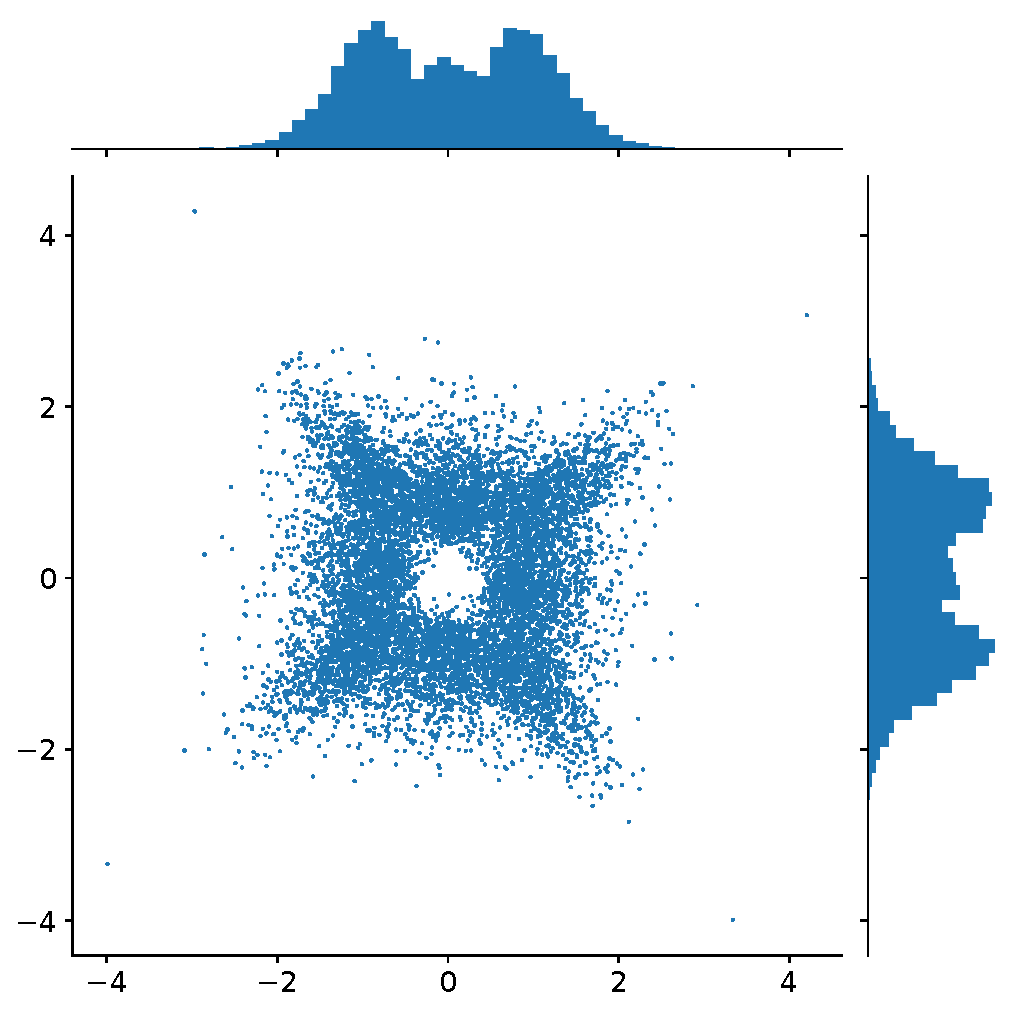
\includegraphics[width=\textwidth]{../Plots/Transformations/ring_joint_marginal_pca.pdf} \quad
\caption{$X_{pca}$}
\end{subfigure}
\begin{subfigure}{0.3\textwidth}
\centering
    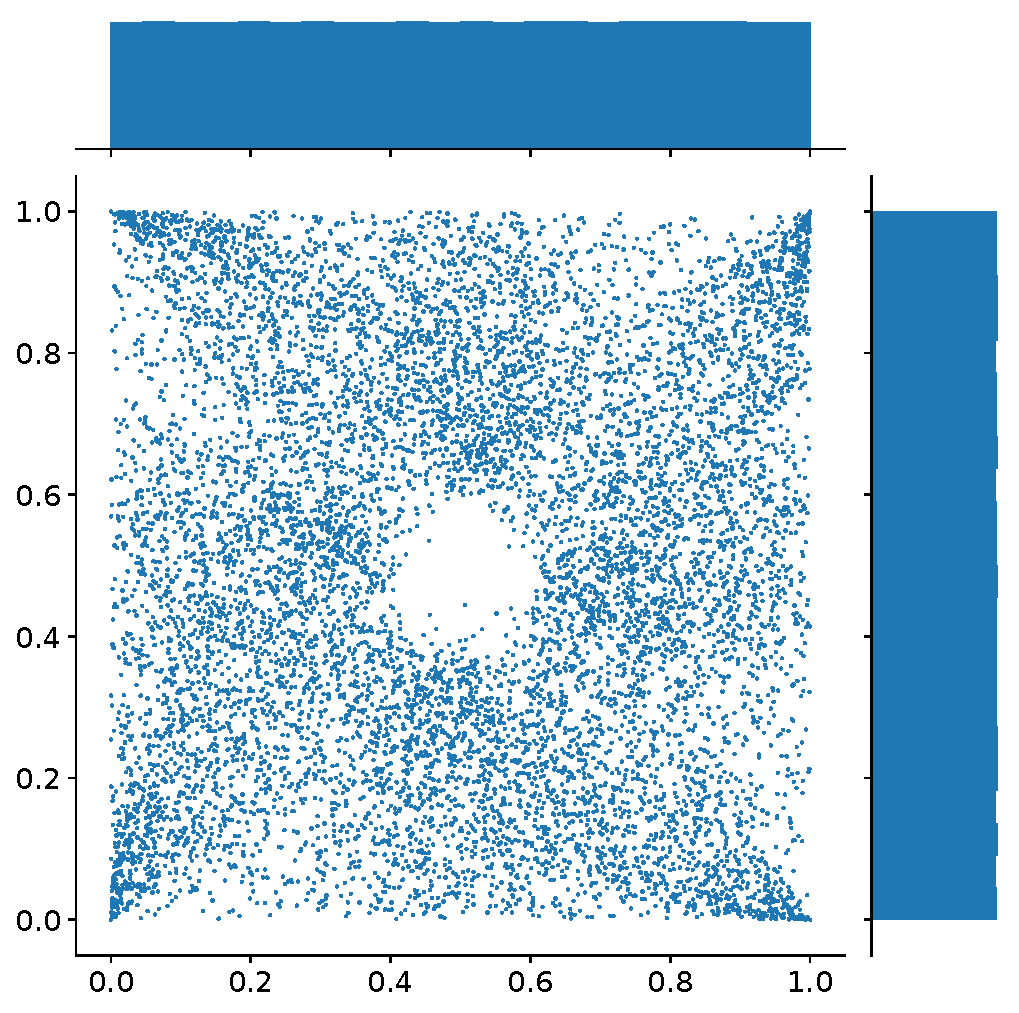
\includegraphics[width=\textwidth]{../Plots/Transformations/ring_joint_marginal_uniform.pdf}
\caption{$X_{uni}$}
\end{subfigure}
\begin{subfigure}{0.3\textwidth}
\centering
    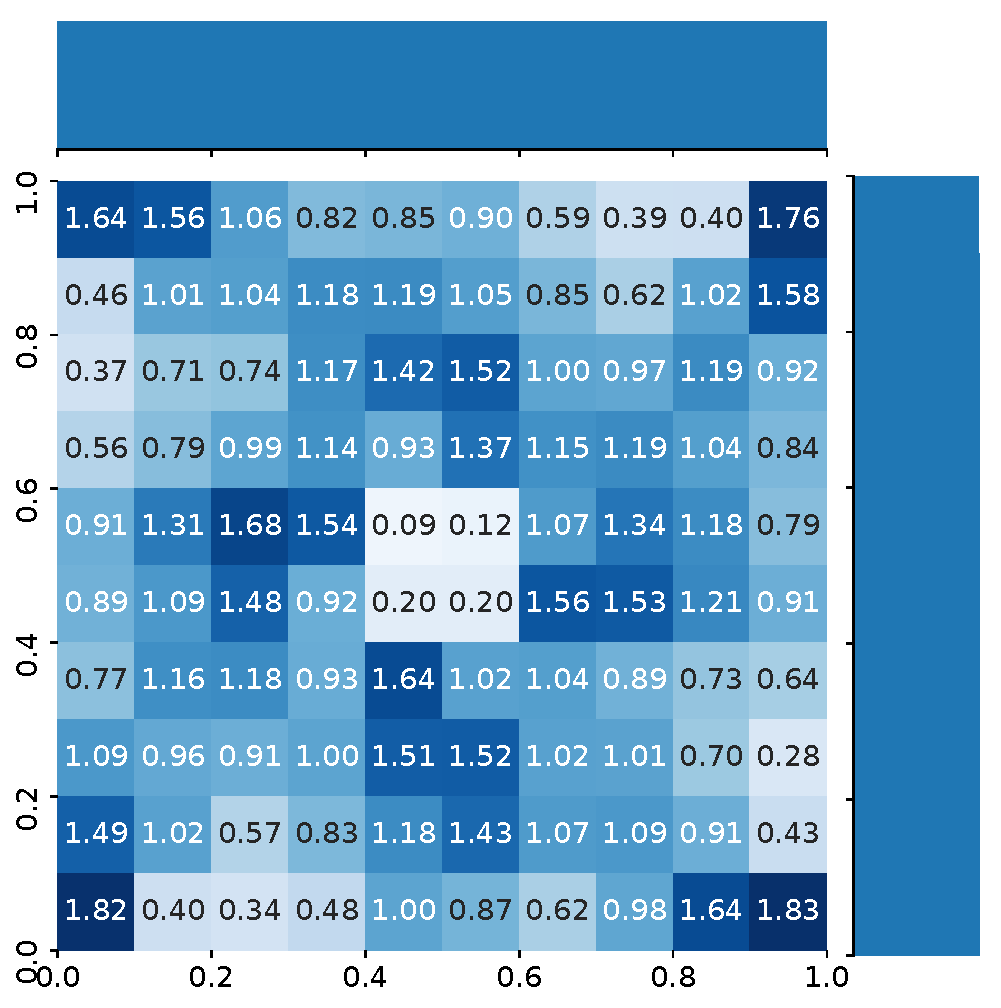
\includegraphics[width=\textwidth]{../Plots/Transformations/ring_discrete_uniform_bn_weights_annotated.pdf}\quad
\caption{BN weights $X_{discrete}$}
\end{subfigure}
\begin{subfigure}{0.3\textwidth}
\centering
    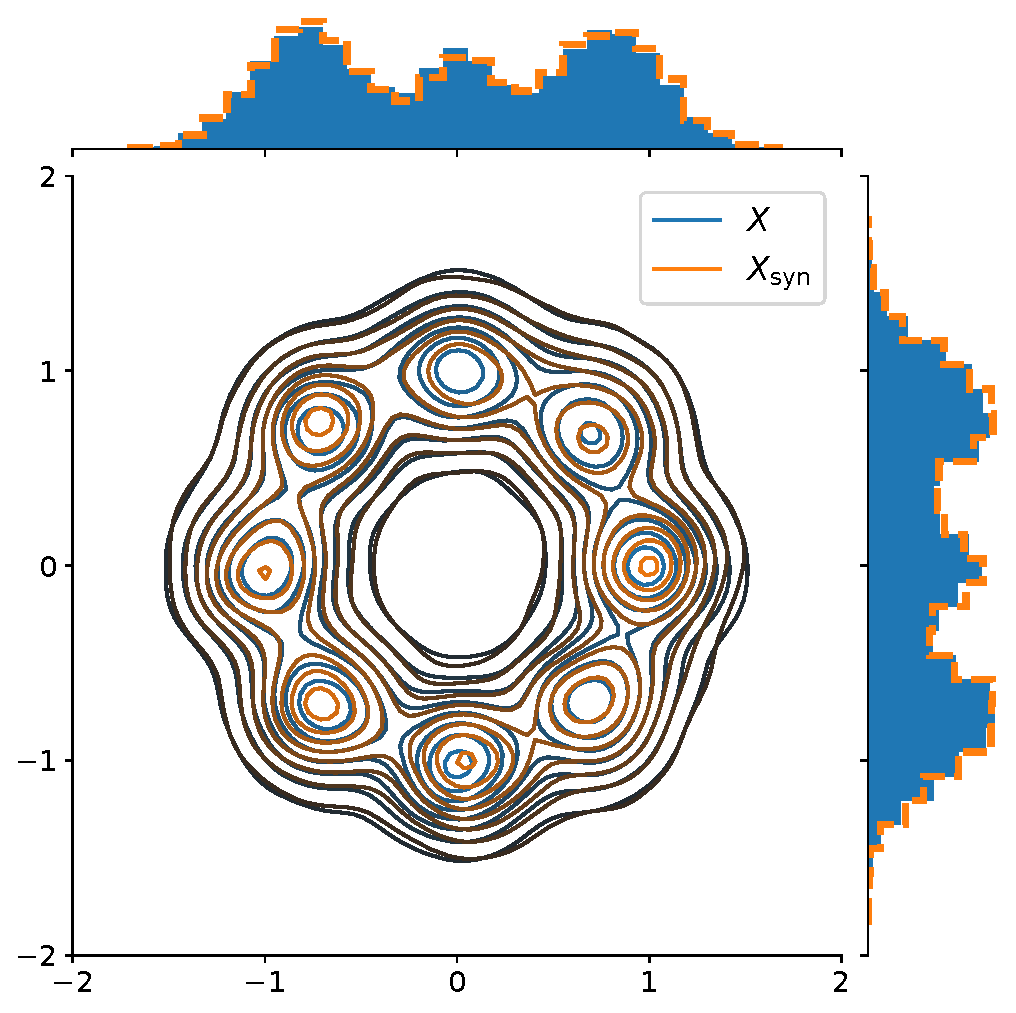
\includegraphics[width=\textwidth]{../Plots/Transformations/ring_joint_marginal_with_sample_contours.pdf}
\caption{$X_{num}$ and $X_{syn}$}
\end{subfigure}
\caption{Numerical transformations example on the ring dataset (a-d), (e) the Copula Bayesian network's weights  for discretized $X_{\rm uniform}$ and (f) a synthetic sample~\cite{AuthorSynthsonic:Data}}
\label{fig:transformation}
\end{figure}


\section{Sampling strategy}
Once Synthsonic has been trained on the data, new samples can be generated in five steps.
\begin{enumerate}
    \item Synthetic samples are generated from the Bayesian Network using forward sampling over the network tree~\cite{Guo2002AInference}.
    \item The discretized numerical features of $X_{discrete}$ are converted back to numerical by adding a small random value from a uniform distribution from (0,0.05) to the bin indices they are in. 
    \item The weights from the discriminative classifier are assigned to all samples. 
    \item The inverse transformations of \ref{sec:Feat_trans} are applied to all features, resulting in a dataset similar to original dataset $X$.
\end{enumerate}